\documentclass[10pt]{beamer}
\usetheme{metropolis}
\usepackage[T1]{fontenc}
\usepackage[utf8]{inputenc}
\usepackage{graphicx}
\usepackage{stmaryrd}

\title{Présentation étude d'incertitudes sur l'équation de Burgers}
\author{Demuth Axel}
\date{\today}

\begin{document}

\maketitle

\section{Introduction}
\begin{frame}{Introduction}
    On étudie l'importance des paramètres influençant la dynamique d'un bouchon de circulation, modélisé par l'équation de Burgers suivante : 

    \begin{equation}
        \frac{\partial \rho}{\partial t} + \frac{\partial}{\partial x} \big(\rho v(\rho)\big) = 0,
        \end{equation}
        avec 
        \begin{equation}
        v(\rho) = v_{\text{max}} \left( 1 - \frac{\rho}{\rho_{\text{max}}} \right),
        \end{equation}
        et 
        \begin{equation}
        \rho(t = 0, x) =
        \begin{cases} 
        \rho_{\text{in}}, & x < x_C, \\
        \rho_{\text{out}}, & x > x_C.
        \end{cases}
    \end{equation}
        
\end{frame}

\section{Analyse Burgers}
\begin{frame}

    Avec le code Burger's fournie nous obtenons ce résultat : 
    \begin{figure}[h!]
        \centering
        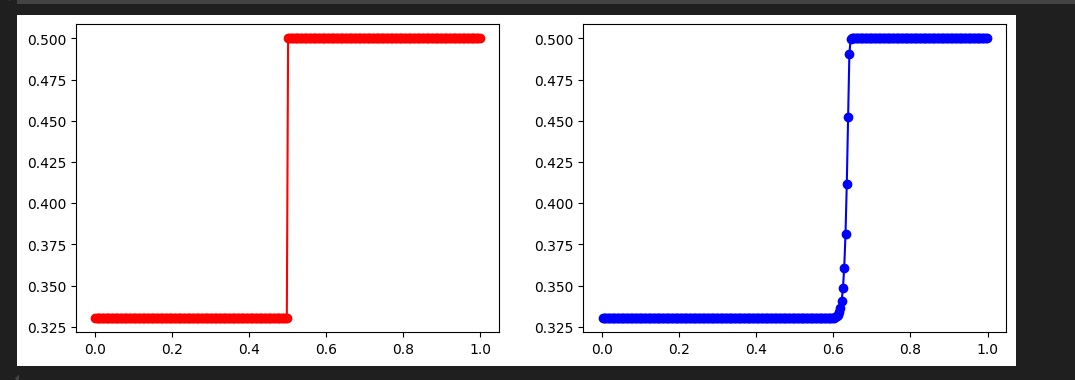
\includegraphics[width=0.8\textwidth]{burger_classique.png} % Remplacez par le chemin de votre image
        \caption{\( \rho_{\text{in}} = U(0.2,0.35)\), \( \rho_{\text{out}} = 0.5 \), \( x_C = 0.5 \), \( v_{\text{max}} = N(0.8,0.35) \)}
        \label{fig:conditions_initiales}
    \end{figure}
    
\end{frame}

\begin{frame}
     On peut aussi regarder les intervalles de confiance par Monte Carlo avec \( \rho_{\text{in}} < \rho_{\text{out}} \): 
        \begin{figure}[h!]
            \centering
            \includegraphics[width=0.8\textwidth]{densité_rin_inf_rout.png} % Remplacez par le chemin de votre image
            \caption{\( \rho_{\text{in}} = U(0.2,0.35)\), \( \rho_{\text{out}} = U(0.5,0.65) \), \( x_C = 0.5 \), \( v_{\text{max}} = N(0.8,0.35) \)}
        \end{figure}
        
\end{frame}


\begin{frame}
    Pour \( \rho_{\text{in}} > \rho_{\text{out}} \): 
       \begin{figure}[h!]
           \centering
           \includegraphics[width=0.8\textwidth]{densité_rin_sup_rout.png} % Remplacez par le chemin de votre image
           \caption{\( \rho_{\text{in}} = U(0.5,0.65)\), \( \rho_{\text{out}} = U(0.2,0.35) \), \( x_C = 0.5 \), \( v_{\text{max}} = N(0.8,0.35) \)}
       \end{figure}
       
\end{frame}

\begin{frame}{Calcul de Limite}
    
    \begin{figure}
        \centering
        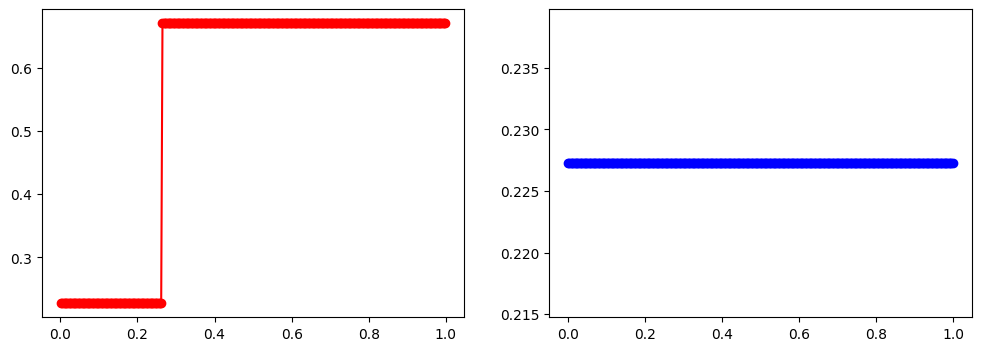
\includegraphics[width=0.8\textwidth]{limite_burgers.png}
        \caption{$\lim_{T \to \infty} \rho_t$}
    \end{figure}
\end{frame}


\begin{frame}{Calcul Espérance,variance,intervalles de confiances}
    Par Monte Carlo, nous obtenons les statistiques suivantes pour le nombre d'unité de Temps nécessaire pour résorber un bouchon: 
    \begin{itemize}
        \item Espérance de \( Y \) : \( 2.8314 \)
        \item Variance de \( Y \) : \( 2.6032 \)
        \item Intervalle de confiance à 95\% : \( (2.5152, 3.1477) \)
    \end{itemize}
    
    Les paramètres utilisés pour la simulation sont: 
    \begin{itemize}
        \item \( v_{\text{max}} = \mathcal{N}(0.7, 0.05) \)
        \item \( \rho_{\text{in}} = U(0.1, 0.5) \)
        \item \( \rho_{\text{out}} = U(0.5, 0.9) \)
        \item \( x_C = U(0.2, 0.8) \)
    \end{itemize}
\end{frame}


\section{Sobol et Métamodèle}

\begin{frame}{Indice de Sobol}
    Soit \( X_i' \) une copie indépendante de \( X_i \), et
    \[
    Y = Q(X_i, X_{-i})
    \]
    \[
    Y^i = Q(X_i, X_{-i}')
    \]
    \[
    Y^{-i} = Q(X_i', X_{-i})
    \]
    
    Nous définissons ensuite :
    
    \[
    S_i = \frac{\text{cov}(Y, Y^i)}{\text{Var}(Y)}
    \]
    et
    \[
    S_i^{\text{tot}} = \frac{\mathbb{E} \left[ (Y - Y^{-i})^2 \right]}{\text{Var}(Y)}
    \]
    

\end{frame}

\begin{frame}{Métamodèle}
    Pour un métamodèle, On essaye d'utiliser le Krigeage en raison du comportement non linéaire complexe de l'équation de Burgers. 
    Le Krigeage permet d'interpoler efficacement ces comportements tout en réduisant le coût computationnel des simulations. 

\end{frame}

\begin{frame}{Conclusion}
    
        En conclusion, Avec l'étude du modèle De Burger's nous pouvons estimer et mieux comprendre le comportement du flux de véhicule et comprendre les différentes importance des paramètres
    

\end{frame}

\end{document}

